\documentclass[12pt, a4paper]{article}

\usepackage[T1]{fontenc}
\usepackage[utf8]{inputenc}
\usepackage[brazil]{babel}
\usepackage{times}
\usepackage{listings}
\usepackage{graphicx}
\graphicspath{ {images/} }
\usepackage{caption}
\usepackage{url}
\usepackage{subcaption}
\usepackage{float}
\usepackage{amsmath}
\usepackage[export]{adjustbox}
\usepackage{tabularx}
\usepackage{dcolumn}
\usepackage{multirow}
\usepackage{booktabs}
\usepackage{indentfirst}
\usepackage{balance}
\usepackage{flushend}
\usepackage{geometry}
\usepackage{float}
\geometry{top=2.0cm, bottom=1.8cm, left=2.3cm, right=2.2cm}

\usepackage{blindtext}
\title{Um Estudo Sobre a Eficiência da Alocação \\ Dinâmica de Slices em Redes 5G}
\author{Aluno: Caio Krauthamer (RA 165457) \\ Orientador: Prof. Edmundo R. M. Madeira \\[0.2cm] Instituto de Computação, Universidade Estadual de Campinas \\ Campinas-SP 13083-852}
\date{Novembro de 2018}

\begin{document}

\tolerance = 999
\sloppy

\maketitle

\section{Resumo}

Devido ao alto número de equipamentos se conectando à rede, e aos diferentes números de \textit{QoS - Quality of Service} que cada usuário necessita, tornando a rede heterogênea, nasceu a rede 5G. Essa nova geração pretende integrar a ela os chamados \textit{"Network Slices"}, que consiste em fatiar a rede em diferentes redes virtuais sob um único substrato físico afim de se garantir diferentes \textit{QoS} para cada tipo de usuário, garantindo elasticidade, flexibilidade, programabilidade e modularização para a rede. Esses \textit{slices} são criados via um orquestrador, que conhecendo o estado atual da rede, redimensiona os \textit{slices} existentes para garantir uma melhor experiência aos usuários. Este projeto visa estudar a alocação dinâmica de dados a serem enviados na rede, que é uma melhora extra além da existência de \textit{slices}, em um cenário de uma quadra de futsal.

\section{Fundamentação Teórica}

As redes 5G se baseiam na quebra das responsabilidades na rede em dois planos: lógica e de dados. O plano lógico (conhecido também como plano de controle) toma as decisões de negócio na transmissão de um pacote, como por exemplo para qual roteador encaminhar um pacote, dado o substrato da rede atual. E o plano de dados, que apenas faz o roteamento de pacotes no substrato da rede, respondendo aos comandos recebidos da camada lógica. Esta divisão de tarefas chama-se \textit{SDN - Software Defined Network}.

Também, a rede sem fio no caminho para o 5G faz uso de \textit{LTE - Long Term Evolution}, na qual divide o quadro de dados a serem enviados em 10 subquadros de duas maneiras: \textit{TDD - Time Division Duplex} e \textit{FDD - Frequency Division Duplex}. A primeira, que será utilizada no experimento, divide o quadro de dados em relação ao tempo, isto é, divide o quadro em fatias, onde cada fatia tem um intervalo de tempo para transmitir. Já a segunda divide o quadro em 10 subquadros de frequências distintas, onde todas as frequências são transmitidas ao mesmo tempo.

Além dessa divisão, cada subquadro, independente da topologia usada, pode, e será neste estudo, dividido em \textit{RB - Resource Blocks}, que é a menor unidade a qual pode ser alocada para um \textit{UE - User Equipment}.

No experimento o quadro da rede LTE foi dividido em 10 subquadros de 1ms cada, que é o  \textit{TTI - Transmission Time Interval}, e cada subquadro dividido em 10 RBs cada, totalizando 100 RBs que podem ser alocados para um UE a cada rodada de transmissão, que dura 10ms. Uma ilustração da divisão do quadro LTE em RBs pode ser vista na Figura \ref{slices}

A cada rodada, o orquestrador recebe os dados do substrato da rede e também os dados que cada UE deseja transmitir naquela rodada, e define qual RB vai transmitir qual dado de qual UE com base nas políticas e prioridades de cada \textit{slice} e o \textit{QoS} que cada dado necessita para ser transmitido.

\begin{figure}[H]
	\centering
	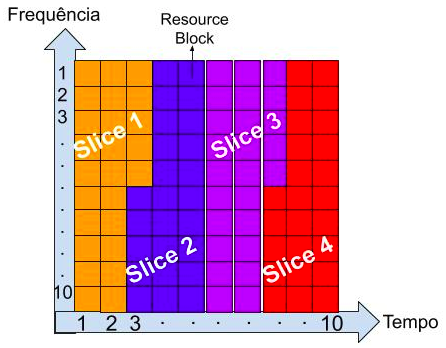
\includegraphics[width=0.8\textwidth, frame]{/home/caio/tcc-slices/ns-3.29/results/slices.png}
	\caption{Exemplo de quadro LTE dividido em slices e RBs}
	\label{slices}
\end{figure}

\section{Arquitetura do Sistema}

\subsection{Descrição do cenário}

O cenário de estudo foi uma quadra de futsal, na qual tinham quatro UEs na quadra, em uma área de 40 x 20 metros, sendo um para cada gol, um para a bola e outro para o juiz. Esses quatro equipamentos faziam transmissão de dados \textit{uplink} e \textit{downlink} FTP para ter informações como bola entrou ou não em um gol e comunicação de ações por parte da central para o juiz da partida. Os demais UEs compunham os espectadores da partida, sendo divididos em quatro setores: norte, sul, leste e oeste, onde norte e sul ficam atrás dos gols e leste e oeste nas laterais dos campos. As dimensões desses setores eram de 15 x 70 metros no setor norte e sul e de 40 x 15 metros nos setores leste e oeste. Uma ilustração de como estes equipamentos estão dispostos no início de cada simulação pode ser encontrado na Figura \ref{estádio}, obtidos usando o simulador NetAnim \cite{netAnim}. Estes usuários fazem \textit{upload} de \textit{streaming} de vídeo UDP, recepção de áudio da narração do jogo em VoIP, envio e recepção de imagens e texto FTP. O principal foco deste estudo é melhorar principalmente a comunicação de equipamentos para um bom andamento da partida e também focar nas necessidades mais comuns dos espectadores do evento, que no caso é o envio de vídeo.

\begin{figure}[H]
	\centering
	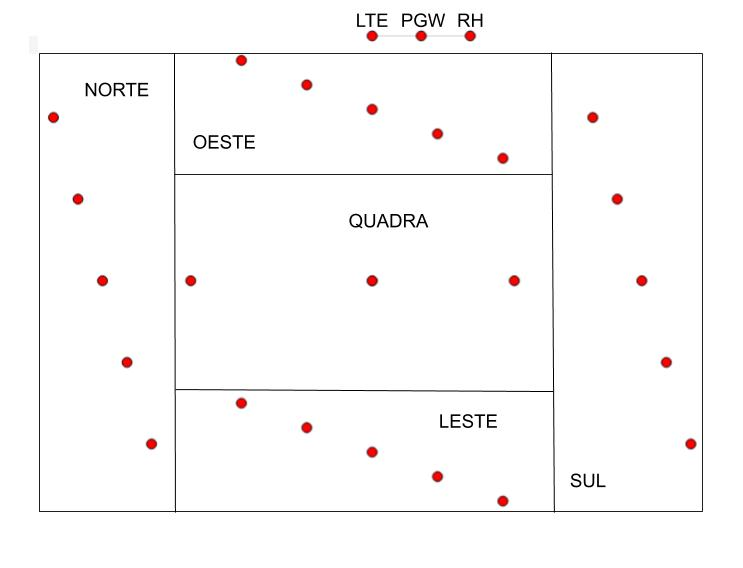
\includegraphics[width=0.8\textwidth, frame]{/home/caio/tcc-slices/ns-3.29/results/estadio.jpg}
	\caption{UEs distribuídos no estádio}
	\label{estádio}
\end{figure}

Dado este cenário foram criados oito \textit{slices}, sendo metade para o \textit{uplink} e a outra metade para o \textit{downlink}. Os \textit{slices} de  \textit{downlink} são os seguintes: 1 - Recepção de dados FTP, 2 - Recepção de áudio VoIP, 3 - Recepção de imagem FTP e 4 - Recepção de texto FTP. Já os de \textit{uplink} são: 11 - Envio de dados FTP, 12 - Envio de \textit{streaming} de vídeo UDP, 13 - Envio de imagens FTP, 14 - Envío de texto FTP. Os RBs foram divididos de tal forma que nos canais de \textit{downlink} 25.2\% foram alocados para o \textit{slice} 1, 24.8\% foram alocados para o 2, 24.8\% foram alocados para o 3 e 25.2\% foram alocados para o 4. Já para o  \textit{uplink} 25.2\% foram alocados para o \textit{slice} 11, 24.8\% foram alocados para o 12, 24.8\% foram alocados para o 13 e 25.2\% foram alocados para o 14.

A prioridade de cada \textit{slice} ficou definida como maior prioridade para os UEs da quadra, já que estes não podem atrasar a partida esperando confirmação de ações durante o jogo, seguido de \textit{streaming} de vídeo UDP, já que essa é uma aplicação que trafega mais dados pela rede, e perdas ou atrasos não constantes de pacotes podem causar travamento do vídeo, além de ser o tipo de tráfego mais requisitado pelos espectadores empatado com a transmissão da narração do jogo por VoIP, seguido de envio e recebimento de imagens e finalizado pelo envio e recebimento de texto, estes dois últimos com menor prioridade, pois são menos comuns no cenário em questão.

Uma consolidação dos \textit{slices}, do tipo de dado trafegado em cada um, a prioridade de cada um, tão quanto a quantidade de UEs transmitindo em cada \textit{slice} podem ser encontrados nas Tabelas \ref{canais downlink} e \ref{canais uplink}. 

\begin{table*}[!htb]
	\setlength{\tabcolsep}{5mm}
	\centering
	\begin{tabular}{c|c|c|c}
		\toprule
		Slice ID & Prioridade & Tipo de tráfego & Quantidade de UEs 
		\\
		\midrule
		1 & 3 & Receção Quadra FTP & 4 (equipamentos da quadra)
		\\
		2 & 2 & Recepção de Áudio VoIP & 15\% dos espectadores
		\\
		3 & 1 & Recepção de Imagem FTP & 15\% dos espectadores
		\\
		4 & 0 & Recepção de Texto FTP & 55\% dos espectadores
		\\
		\bottomrule
	\end{tabular}
	\caption{Slices de Downlink e UEs na rede}
	\label{canais downlink}
\end{table*}

\begin{table*}[!htb]
	\setlength{\tabcolsep}{5mm}
	\centering
	\begin{tabular}{c|c|c|c}
		\toprule
		Slice ID & Prioridade & Tipo de tráfego & Quantidade de UEs 
		\\
		\midrule
		11 & 3 & Envio Quadra FTP & 4 (equipamentos da quadra)
		\\
		12 & 2 & Envio de Vídeo UDP & 15\% dos espectadores
		\\
		13 & 1 & Envio de Imagem FTP & 15\% dos espectadores
		\\
		14 & 0 & Envio de Texto FTP & 55\% dos espectadores
		\\
		\bottomrule
	\end{tabular}
	\caption{Slices de Uplink e UEs na rede}
	\label{canais uplink}
\end{table*}

\subsection{Descrição dos Elementos da Rede e seu Algoritmo}

A rede estava configurada com os UEs conectados a uma antena LTE que se conectava a um \textit{PGW - Packet Data Network Gateway} que por sua vez se conectava a um \textit{RH - remote host}, que representava a outra extremidade da conexão, que iria receber os dados enviados pelos espectadores e enviar os dados aos espectadores, estes três elementos estão separados por dez metros uns dos outros e podem ser encontrados na ordem mencionada, da esquerda para direita, na Figura \ref{estádio}.

O cenário foi comparado em duas topologias: alocação de RBs de forma estática e de forma dinâmica. Para forma estática, em uma dada rodada de transmissão um tipo de serviço poderia apenas utilizar RBs definidos previamente para aquele tipo de aplicação, sendo RBs inutilizados durante aquela rodada pela aplicação, sendo desperdiçados. Já para a alocação dinâmico, caso um RB não viesse a ser utilizado em uma rodada por uma aplicação, então este era cedido a outra aplicação seguindo a ordem de prioridade definida no orquestrador. O modelo estático é o modo usual de redes 5G dividas em \textit{slices}, necessitando apenas do orquestrador saber quais RBs estão alocados para cada \textit{vertical}, através de uma matriz de alocação, entretanto o modelo dinâmico necessita de um código de um orquestrador mais complexo, que além de fazer e necessitar tudo que o estático faz e tem, também irá armazenar a prioridade de cada \textit{slice}, bem como verificar a cada rodada a melhor forma de preencher todos RB com dados, mas sempre respeitando a prioridade de cada tipo de aplicação.

Para isso, utilizou-se a implementação em ~\cite{rezende3}. Esta implementação, de forma simplificada, consiste em um Descritor de \textit{Slices} (DS), que contém os fluxos registrados em cada \textit{slice}, suas políticas e prioridades, uma Matriz de Alocação para cada canal (MAD \& MAU), que armazena a distribuição de recursos aos \textit{slices}, ou seja,  se um \textit{slice} receber três RB, então três das N posições disponíveis no MAD/MAU serão alocadas para esse \textit{slice}, onde N é o número de RBs disponibilizados ao controlador SDN. No MAD/MAU, os identificadores dos \textit{slices} são distribuídos de acordo com a alocação computada pelo orquestrador, um Mapa de Alocação (MA), que é gerado pelo orquestrador, que recebe DS e MAD/MAU e mapeia os valores de MAD/MAU em \textit{resource blocks} de rádio, então, obtém-se um mapa onde a chave é o RB e o valor é o identificador do \textit{slice}. Ligando tudo: o DS descreve quais as necessidades e quais são cada \textit{slice}, o MAD/MAU armazena quantos RBs estarão disponíveis para cada \textit{slice} e por fim o MA armazena um mapeando real de qual(is) RB(s) serão utilizados por qual \textit{slice} na atual rodada de transmissão.

\section{Avaliação de Desempenho}

Foram feitas execuções para cenários com 20, 24, 28 e 32 UEs no simulador ns-3 \cite{ns3}, tanto para o cenário estático quanto para o cenário dinâmico. Para cada cenário foram executadas dez vezes cada simulação com diferentes \textit{seeds} e por dois minutos. Os resultados foram colhidos para as métricas de \textit{delay}, \textit{jitter}, \textit{throughput} e \textit{lost packets}, calculando a média das dez execuções e seu desvio padrão. Os pontos em vermelho se referem às execuções com alocação de RBs de forma estática e os em azul, dinâmica.

Nas Figuras \ref{delay1}, \ref{delay2}, \ref{delay3}, \ref{delay4}, \ref{delay11}, \ref{delay12}, \ref{delay13} e \ref{delay14} encontram-se as imagens respectivas ao delay em cada \textit{slice}.

Nas Figuras \ref{jitter1}, \ref{jitter2}, \ref{jitter3}, \ref{jitter4}, \ref{jitter11}, \ref{jitter12}, \ref{jitter13} e \ref{jitter14} encontram-se as imagens respectivas ao jitter em cada \textit{slice}.   

Nas Figuras \ref{lost_packets1}, \ref{lost_packets2}, \ref{lost_packets3}, \ref{lost_packets4}, \ref{lost_packets11}, \ref{lost_packets12}, \ref{lost_packets13} e \ref{lost_packets14} encontram-se as imagens respectivas à porcentagem de pacotes perdidos em cada \textit{slice}.

Nas Figuras \ref{throughput1}, \ref{throughput2}, \ref{throughput3}, \ref{throughput4}, \ref{throughput11}, \ref{throughput12}, \ref{throughput13} e \ref{throughput14} encontram-se as imagens respectivas à vazão em cada \textit{slice}.

\begin{figure}[H]
	\centering
	\includegraphics[width=0.8\textwidth, frame]{/home/caio/tcc-slices/ns-3.29/results/graphics/compound/delay/slice_01_quadra_ftp.png}
	\caption{Delay no Slice 1}
	\label{delay1}
\end{figure}

\begin{figure}[H]
	\centering
	\includegraphics[width=0.8\textwidth, frame]{/home/caio/tcc-slices/ns-3.29/results/graphics/compound/delay/slice_02_espectadores_voip_audio.png}
	\caption{Delay no Slice 2}
	\label{delay2}
\end{figure}

\begin{figure}[H]
	\centering
	\includegraphics[width=0.8\textwidth, frame]{/home/caio/tcc-slices/ns-3.29/results/graphics/compound/delay/slice_03_espectadores_ack_ftp_imagem.png}
	\caption{Delay no Slice 3}
	\label{delay3}
\end{figure}

\begin{figure}[H]
	\centering
	\includegraphics[width=0.8\textwidth, frame]{/home/caio/tcc-slices/ns-3.29/results/graphics/compound/delay/slice_04_espectadores_ack_ftp_texto.png}
	\caption{Delay no Slice 4}
	\label{delay4}
\end{figure}

\begin{figure}[H]
	\centering
	\includegraphics[width=0.8\textwidth, frame]{/home/caio/tcc-slices/ns-3.29/results/graphics/compound/delay/slice_11_quadra_ftp.png}
	\caption{Delay no Slice 11}
	\label{delay11}
\end{figure}

\begin{figure}[H]
	\centering
	\includegraphics[width=0.8\textwidth, frame]{/home/caio/tcc-slices/ns-3.29/results/graphics/compound/delay/slice_12_espectadores_udp_video.png}
	\caption{Delay no Slice 12}
	\label{delay12}
\end{figure}

\begin{figure}[H]
	\centering
	\includegraphics[width=0.8\textwidth, frame]{/home/caio/tcc-slices/ns-3.29/results/graphics/compound/delay/slice_13_espectadores_ftp_imagem.png}
	\caption{Delay no Slice 13}
	\label{delay13}
\end{figure}

\begin{figure}[H]
	\centering
	\includegraphics[width=0.8\textwidth, frame]{/home/caio/tcc-slices/ns-3.29/results/graphics/compound/delay/slice_14_espectadores_ftp_texto.png}
	\caption{Delay no Slice 14}
	\label{delay14}
\end{figure}

\begin{figure}[H]
	\centering
	\includegraphics[width=0.8\textwidth, frame]{/home/caio/tcc-slices/ns-3.29/results/graphics/compound/jitter/slice_01_quadra_ftp.png}
	\caption{Jitter no Slice 1}
	\label{jitter1}
\end{figure}

\begin{figure}[H]
	\centering
	\includegraphics[width=0.8\textwidth, frame]{/home/caio/tcc-slices/ns-3.29/results/graphics/compound/jitter/slice_02_espectadores_voip_audio.png}
	\caption{Jitter no Slice 2}
	\label{jitter2}
\end{figure}

\begin{figure}[H]
	\centering
	\includegraphics[width=0.8\textwidth, frame]{/home/caio/tcc-slices/ns-3.29/results/graphics/compound/jitter/slice_03_espectadores_ack_ftp_imagem.png}
	\caption{Jitter no Slice 3}
	\label{jitter3}
\end{figure}

\begin{figure}[H]
	\centering
	\includegraphics[width=0.8\textwidth, frame]{/home/caio/tcc-slices/ns-3.29/results/graphics/compound/jitter/slice_04_espectadores_ack_ftp_texto.png}
	\caption{Jitter no Slice 4}
	\label{jitter4}
\end{figure}

\begin{figure}[H]
	\centering
	\includegraphics[width=0.8\textwidth, frame]{/home/caio/tcc-slices/ns-3.29/results/graphics/compound/jitter/slice_11_quadra_ftp.png}
	\caption{Jitter no Slice 11}
	\label{jitter11}
\end{figure}

\begin{figure}[H]
	\centering
	\includegraphics[width=0.8\textwidth, frame]{/home/caio/tcc-slices/ns-3.29/results/graphics/compound/jitter/slice_12_espectadores_udp_video.png}
	\caption{Jitter no Slice 12}
	\label{jitter12}
\end{figure}

\begin{figure}[H]
	\centering
	\includegraphics[width=0.8\textwidth, frame]{/home/caio/tcc-slices/ns-3.29/results/graphics/compound/jitter/slice_13_espectadores_ftp_imagem.png}
	\caption{Jitter no Slice 13}
	\label{jitter13}
\end{figure}

\begin{figure}[H]
	\centering
	\includegraphics[width=0.8\textwidth, frame]{/home/caio/tcc-slices/ns-3.29/results/graphics/compound/jitter/slice_14_espectadores_ftp_texto.png}
	\caption{Jitter no Slice 14}
	\label{jitter14}
\end{figure}

\begin{figure}[H]
	\centering
	\includegraphics[width=0.8\textwidth, frame]{/home/caio/tcc-slices/ns-3.29/results/graphics/compound/lost_packets/slice_01_quadra_ftp.png}
	\caption{Pacotes Perdidos no Slice 1}
	\label{lost_packets1}
\end{figure}

\begin{figure}[H]
	\centering
	\includegraphics[width=0.8\textwidth, frame]{/home/caio/tcc-slices/ns-3.29/results/graphics/compound/lost_packets/slice_02_espectadores_voip_audio.png}
	\caption{Pacotes Perdidos no Slice 2}
	\label{lost_packets2}
\end{figure}

\begin{figure}[H]
	\centering
	\includegraphics[width=0.8\textwidth, frame]{/home/caio/tcc-slices/ns-3.29/results/graphics/compound/lost_packets/slice_03_espectadores_ack_ftp_imagem.png}
	\caption{Pacotes Perdidos no Slice 3}
	\label{lost_packets3}
\end{figure}

\begin{figure}[H]
	\centering
	\includegraphics[width=0.8\textwidth, frame]{/home/caio/tcc-slices/ns-3.29/results/graphics/compound/lost_packets/slice_04_espectadores_ack_ftp_texto.png}
	\caption{Pacotes Perdidos no Slice 4}
	\label{lost_packets4}
\end{figure}

\begin{figure}[H]
	\centering
	\includegraphics[width=0.8\textwidth, frame]{/home/caio/tcc-slices/ns-3.29/results/graphics/compound/lost_packets/slice_11_quadra_ftp.png}
	\caption{Pacotes Perdidos no Slice 11}
	\label{lost_packets11}
\end{figure}

\begin{figure}[H]
	\centering
	\includegraphics[width=0.8\textwidth, frame]{/home/caio/tcc-slices/ns-3.29/results/graphics/compound/lost_packets/slice_12_espectadores_udp_video.png}
	\caption{Pacotes Perdidos no Slice 12}
	\label{lost_packets12}
\end{figure}

\begin{figure}[H]
	\centering
	\includegraphics[width=0.8\textwidth, frame]{/home/caio/tcc-slices/ns-3.29/results/graphics/compound/lost_packets/slice_13_espectadores_ftp_imagem.png}
	\caption{Pacotes Perdidos no Slice 13}
	\label{lost_packets13}
\end{figure}

\begin{figure}[H]
	\centering
	\includegraphics[width=0.8\textwidth, frame]{/home/caio/tcc-slices/ns-3.29/results/graphics/compound/lost_packets/slice_14_espectadores_ftp_texto.png}
	\caption{Pacotes Perdidos no Slice 14}
	\label{lost_packets14}
\end{figure}

\begin{figure}[H]
	\centering
	\includegraphics[width=0.8\textwidth, frame]{/home/caio/tcc-slices/ns-3.29/results/graphics/compound/throughput/slice_01_quadra_ftp.png}
	\caption{Vazão no Slice 1}
	\label{throughput1}
\end{figure}

\begin{figure}[H]
	\centering
	\includegraphics[width=0.8\textwidth, frame]{/home/caio/tcc-slices/ns-3.29/results/graphics/compound/throughput/slice_02_espectadores_voip_audio.png}
	\caption{Vazão no Slice 2}
	\label{throughput2}
\end{figure}

\begin{figure}[H]
	\centering
	\includegraphics[width=0.8\textwidth, frame]{/home/caio/tcc-slices/ns-3.29/results/graphics/compound/throughput/slice_03_espectadores_ack_ftp_imagem.png}
	\caption{Vazão no Slice 3}
	\label{throughput3}
\end{figure}

\begin{figure}[H]
	\centering
	\includegraphics[width=0.8\textwidth, frame]{/home/caio/tcc-slices/ns-3.29/results/graphics/compound/throughput/slice_04_espectadores_ack_ftp_texto.png}
	\caption{Vazão no Slice 4}
	\label{throughput4}
\end{figure}

\begin{figure}[H]
	\centering
	\includegraphics[width=0.8\textwidth, frame]{/home/caio/tcc-slices/ns-3.29/results/graphics/compound/throughput/slice_11_quadra_ftp.png}
	\caption{Vazão no Slice 11}
	\label{throughput11}
\end{figure}

\begin{figure}[H]
	\centering
	\includegraphics[width=0.8\textwidth, frame]{/home/caio/tcc-slices/ns-3.29/results/graphics/compound/throughput/slice_12_espectadores_udp_video.png}
	\caption{Vazão no Slice 12}
	\label{throughput12}
\end{figure}

\begin{figure}[H]
	\centering
	\includegraphics[width=0.8\textwidth, frame]{/home/caio/tcc-slices/ns-3.29/results/graphics/compound/throughput/slice_13_espectadores_ftp_imagem.png}
	\caption{Vazão no Slice 13}
	\label{throughput13}
\end{figure}

\begin{figure}[H]
	\centering
	\includegraphics[width=0.8\textwidth, frame]{/home/caio/tcc-slices/ns-3.29/results/graphics/compound/throughput/slice_14_espectadores_ftp_texto.png}
	\caption{Vazão no Slice 14}
	\label{throughput14}
\end{figure}

Para a métrica de \textit{delay} é interessante notar como em praticamente todos os \textit{slices} o modelo dinâmico foi superior ao estático. O único caso em que a média na simulação estática foi inferior a dinâmica foi no \textit{slice} 14, que lida com o envio de mensagens de texto. Isso provavelmente ocorreu pois em algumas rodadas de transmissão que sobrariam RBs não utilizados por outros \textit{slices} que acabaram sendo realocados para outros com maior prioridade no modelo dinâmico (já que o \textit{slice} em questão tem a prioridade mais baixa). Isto deve ter causado um maior uso da rede nestes momentos, explicando o por que para este \textit{slice} em específico a média do atraso ser um pouco superior no modelo dinâmico. Também, nota-se que para o \textit{slice} em questão, mesmo com uma média superior no modelo proposto, os valores do atraso médio dos pacotes estão dentro do intervalo de desvio padrão do modelo estático, mostrando que mesmo obtendo um resultado médio pouco superior, este já estava previsto pelo desvio padrão do modelo estático.  Pelo mesmo motivo que causou um maior atraso aos pacotes do \textit{slice} 14 podemos atribuir a razão pela qual outros \textit{slices} tiveram um resultado superior: no cenário dinâmico, sempre que há dado para transmitir e há RBs disponíveis, então esse dado era transmitido, causando assim uma diminuição no atraso médio de cada pacote. Por último, é interessante notar como no modelo proposto os resultados tendem a ser mais uniformes, isto é, o desvio padrão apresentado pelo modelo estático se mostrou, na maioria dos \textit{slices}, ser superior ou pelo menos igual ao desvio padrão apresentado pelo modelo dinâmico.

Já para o \textit{jitter}, que representa a variação no atraso de entrega de pacotes, pode-se notar que o modelo proposto foi pelo menos melhor em todos os \textit{slices}, independente do número de de usuários na rede. Isso é explicado pelo mesmo fato da melhora do atraso médio dos pacotes na maioria dos \textit{slices}: como só há RBs em uma rodada de transmissão sem dados quando não há usuários suficientes desejando transmitir dados, isso faz a variação no atraso médio de pacotes cair, já que agora usuários, que poderiam ter que esperar uma rodada de transmissão inteira para requisitar novamente o envio de seus dados, podem enviar seus pacotes imediatamente, causando a diminuição do \textit{jitter}. Com o enfoque principal do estudo, é relevante notar que para o envio de dados dos dispositivos situados dentro da quadra, tão como espectadores enviando vídeo, tiveram uma redução considerável do \textit{jitter}, chegando em valores entre 15 e 50\%, isso para os equipamentos da quadra mostra uma conexão mais estável e para o \textit{streaming} de vídeo uma reprodução mais suave por quem a esteja consumindo. Contudo, a métrica em questão passou a dar enfoque em um problema, que é a rede passar a ser muito sobrecarregada quando o número de usuários passa a ser grande demais, causando instabilidade e resultados imprevisíveis, como exemplo da medida para 32 UEs nos  \textit{slices} 3, 12 e 14, ilustrados nas Figuras \ref{jitter3}, \ref{jitter12} e \ref{jitter14}, onde as medidas feitas com a maior quantidade de UEs mostrou um resultado fora do padrão apresentado por execuções com menos equipamentos.

Observando a porcentagem de pacotes perdidos nota-se que os dados já não são tão uniformes: na maioria dos \textit{slices} em que a solução foi aplicada diminuiu a perda de pacotes e ao mesmo tempo há poucos \textit{slices} que aumentou. No geral, independente do cenário, a perda de pacotes sempre se manteve abaixo de um valor aceitável, de no máximo 15\%, porém vale ressaltar que no geral houve uma diminuição da perda de pacotes. Todavia, um dos \textit{slices} no qual houve um aumento da perda de pacotes está um dos \textit{slices} que é o que menos deve-se tolerar perda, que é o \textit{slice} 1, representado pela Figura \ref{lost_packets1}, onde houve um aumento considerável da perda de pacotes para os cenários com menos UEs, e um aumento mais razoável nos cenários com mais UEs. Apesar deste resultado ir na contra-mão dos resultados esperados e previstos, vale ressaltar que ainda assim a média da porcentagem de pacotes perdidos está abaixo da metade do valor máximo tolerável, o que não apresenta uma situação alarmante, porém mostra-se uma situação de atenção. Por fim, o mesmo problema que ficou visível ao se analisar o  \textit{jitter} se mostrou nesta métrica também: nos \textit{slices} 3, 12, e 14, representados pelas Figuras \ref{lost_packets3}, \ref{lost_packets12} e \ref{lost_packets14}, nota-se a imprevisibilidade dos dados colhidos ao se aumentar muito o número de usuários na rede. Vale ressaltar que os mesmos \textit{slices} que apresentaram tal instabilidade ao se olhar o \textit{jitter} foram os que apresentaram instabilidade na métrica avaliada por hora.

Por último, resta-se analisar a vazão de dados na rede. Para esta métrica, com ressalvas nos \textit{slices} 4 e 14, onde com 32 UEs foi apresentada uma ínfima diminuição da vazão, pode-se afirmar que o modelo proposto pelo menos melhorou a vazão de dados na rede. Isso ocorreu pelo mesmo motivo já citado: RBs que poderiam ficar inutilizados durante uma rodada de transmissão são cedidos a outros \textit{slices} que tem dados para serem transmitidos naquele momento, sempre respeitando as políticas de prioridade dentre eles. Isso faz com que a vazão de dados na rede aumente, pois dados que uma vez no modelo estático precisam esperar a próxima rodada de transmissão para transmitir os pacotes, no modelo dinâmico esses dados podem ser transmitidos na rodada atual caso haja RBs disponíveis, inutilizados por outros slices. Vale ressaltar, que como enfoque do estudo, os slices 1, 11, e 12, que representam a comunicação de equipamentos de dentro da quadra e de \textit{streaming} de vídeo, tiveram uma alta melhora na vazão, chegando em valores de até 30\% para o slice 1, 20\% para o slice 11 e 10\% para o slice 14, que se mostra numa melhora da \textit{QoS} daquele \textit{vertical}.

\section{Conclusão e Trabalhos futuros}

Ao fim de todas as simulações e análise de dados feitas, é possível observar que no futuro da próxima geração de telefonia móvel teremos uma divisão da rede em dois planos: lógico e de dados. O grande avanço das redes 5G será no plano lógico, que será feito via \textit{software}, no qual possibilitará um fatiamento da rede, onde cada fatia irá se preocupar com a \textit{quality of service} de um único \textit{vertical}. Nesse estudo foi analisada uma proposta que visa dinamizar ainda mais essa nova camada, a fim de aproveitar ao máximo o que ela tem a oferecer. Observando os resultados de simulações dos dois cenários, utilizando um escalonamento de dados aos RBs de forma dinâmica e outro estática, pode-se comprovar que, na grande maioria dos casos, a solução proposta oferece uma grande melhora na transmissão de dados na rede e nos poucos casos que há alguma piora, esta passa a ser pouco importante ou ser uma piora muito insignificante ao ponto de invalidar a solução estudada.

Com tudo dito, vale ressaltar que durante este estudo certos empecilhos ocorreram, principalmente quando se simulou a rede com um número maior de UEs, sendo testado para casos com 44, 48, 52 e 56 equipamentos, no qual a rede ficou estressada a um ponto que os resultados eram imprevisíveis e nem sempre se observava ganho ao comparar os dois modelos vistos. Como futuro estudo fica aberto a inserção de uma nova antena LTE, a fim de dividir a carga de dados a ser transmitida pelos diferentes usuários, possibilitando assim um maior número de espectadores na arena onde o evento irá ocorrer. Também, pode ser estendido o caso de uso no qual há redimensionamento dos RBs alocados aos \textit{slices} durante a simulação, visando atender momentos que venham a ter um pico de tráfego em algum dos slices.

\addcontentsline{toc}{section}{Referências}
\begin{thebibliography}{9}

\bibitem{kaloxylos} 
Alexandros Kaloxylos. A Survey and an Analysis of Network Slicing in 5G Networks, 2018.

\bibitem{afolabi} 
Ibrahim Afolabi, Tarik Taleb, Konstantinos Samdanis, Adlen Ksentini, Hannu Flinck. Network Slicing and Softwarization: 
A Survey on Principles, Enabling Technologies, and Solutions, 2018.

\bibitem{foukas}
Xenofon Foukas. Georgios Patounas, Ahmed Elmokashfi, Mahesh K. Marina. Network Slicing in 5G: Survey and Challenges, 2017.

\bibitem{rezende} 
Pedro H. A. Rezende, Edmundo R. M. Madeira. An adaptive network slicing for LTE Radio Access Networks, 2018.

\bibitem{rezende2}
Pedro H. A. Rezende, Edmundo R. M. Madeira. Um componente de network slicing para o suporte de multi-inquilinos nas RANs do LTE, 2018.

\bibitem{rezende3}
Pedro H. A. Rezende, Edmundo R. M. Madeira. NS-ENFORCER: Enforcing Network Slicing on LTE Access Networks, 2019.

\bibitem{ns3}
ns-3: A Discrete-Event Network Simulator. https://www.nsnam.org/

\bibitem{netAnim}
NetAnim: An Offline Animator. https://www.nsnam.org/wiki/NetAnim

\end{thebibliography}

\end{document}